\documentclass[11pt,a4paper]{article}
\usepackage{fontspec}
\setmainfont[BoldFont=cmunbx.otf,ItalicFont=cmunti.otf,BoldItalicFont=cmunbi.otf]{cmunrm.otf}
\usepackage[russian]{babel}
\usepackage[margin=24mm]{geometry}
\usepackage{amsmath,booktabs,longtable,array,graphicx,hyperref}
\widowpenalty=10000
\clubpenalty=10000
\hypersetup{colorlinks=true,urlcolor=blue}
\begin{document}
\title{Как оптимизация прогноза досмотра меняет рекомендации KION}
\author{}
\date{25 октября 2026 года}
\maketitle

% REPORT_BODY_BEGIN
\emph{Предсказание следующего фильма, модель досмотра и дополнительное обучение рекомендателя.}

Можно ли улучшить рекомендации, если после обучения на следующем просмотре оптимизировать прогноз досмотра? После дополнительного обучения модель стала выбирать фильмы с более высоким предсказанным досмотром, но хуже ранжировать фактический следующий выбор пользователя. Лучшее качество осталось у модели с дополнительными признаками до обучения по награде. Поправка награды на средний досмотр фильма дала меньшую потерю качества, чем прямой прогноз досмотра, во всех трёх проверенных парах запусков.

\section{Данные и оценка}

Использован открытый KION: взаимодействия пользователей, каталог и пользовательские признаки с марта по август 2021 года. Объектом рекомендации служит фильм или сериал. Повторные просмотры одного фильма пользователем объединены в одну запись. Как при этом рассчитан итоговый процент просмотра, в описании данных не уточняется. Дата относится к последнему взаимодействию, а длительность объединяет просмотры этого фильма данным пользователем. Поэтому строку нельзя считать отдельной сессией, а порядок дат не восстанавливает полную историю событий.

Данные разделены по времени. Периоды обучения, оценки и тестовой части указаны в разделе 9. При оценке следующего фильма история зафиксирована до начала оценочного периода и содержит не более 63 прежних объектов. Фильм, просмотренный в тот же день, что и целевой, не добавляется в историю: по записям нельзя определить порядок просмотров внутри дня.

Общее сравнение выполнено на 65 536 запросах от 53 024 пользователей. Целями служат фильмы первого дня активности пользователя в оценочной неделе. Несколько фильмов одного дня образуют отдельные запросы с общей историей; их порядок внутри дня неизвестен. История, динамические признаки и кандидаты зафиксированы на начало оценочного периода; популярность рассчитана за предыдущие семь дней. Это расширение использованной при разработке выборки, а не независимый тест: 16 384 прежних прогноза дополнены 49 152 новыми. Веса моделей не менялись.

Для каждого запроса отбираются 1024 фильма-кандидата. Набор собирается из прогнозов модели следующего фильма (GPT), популярных за предыдущие семь дней фильмов и ItemKNN, который ищет фильмы, просмотренные одними и теми же пользователями. Источники добавляют соответственно 512, 256 и 256 разных фильмов после исключения дубликатов между источниками. Правильный ответ специально не вставляется, ранее просмотренные фильмы не исключаются. Набор содержит наблюдаемый следующий фильм примерно в 82\% запросов. Если фактический следующий фильм отсутствует в словаре модели или не попал в кандидаты, запрос учитывается в оценке с нулевым результатом.

\newpage

\section{Как устроена система}

Сначала GPT архитектуры GPT-2 учится предсказывать следующий фильм по истории. Входная последовательность содержит не более 64 токенов: начальный токен BOS и до 63 последних объектов истории. По этой истории модель предсказывает следующий фильм. Сам фильм во вход не включается. Один подготовленный пример содержит историю пользователя до дня целевого просмотра и один целевой объект. Одному пользователю могут соответствовать несколько примеров. Представления фильмов дополнены признаками каталога, включая текст и участников. Пользовательские признаки входят в начальный токен. Модель обучена на \textbf{3 477 437 подготовленных примерах за две полные эпохи}. После этого GPT и таблица представлений фильмов заморожены: их веса больше не меняются.

Представления GPT поступают в три отдельно обученные ранжирующие головы. Это небольшие сети, которые меняют порядок кандидатов. Каждая добавляет поправку к исходной оценке GPT. A использует представления истории и фильма, оценку GPT и популярность за семь дней. B сохраняет входы A и добавляет статистику популярности, досмотра и внешнего интереса. C сохраняет входы B и добавляет соответствие интересам пользователя, признаки связанных работ и прогресса просмотра серии.

\textbf{Каждая голова обучена на 262 144 выбранных примерах за три эпохи.} На обучающем примере фактический следующий фильм сравнивается с 31 заранее выбранным другим кандидатом. Оценка проводится на полном наборе кандидатов. Головы обучены независимо при общем порядке данных и настройках.

Состав признаков каждой модели и способы их расчёта приведены в разделе 8.

\section{Как добавление признаков меняло качество}

Основная метрика MAP@10 оценивает позицию наблюдаемого следующего фильма. Вклад запроса равен \(1/\mathrm{rank}\), если этот фильм вошёл в первые десять позиций, и нулю в остальных случаях.

Сначала сравним GPT и три ранжирующие модели. Каждый следующий вариант от A к B и от B к C сохраняет признаки предыдущего и добавляет новые. Все модели оценены на одинаковых запросах и кандидатах. Значения округлены. Точные результаты доступны в \href{https://github.com/suprend/kion-rl-recsys/blob/0154a495704c461adebc281de68d63a652946ec1/report-latex/evaluation64k.json}{результатах расширенной оценки}.

\begin{center}
\begin{tabular}{lr}
\toprule
Модель & MAP@10 \\
\midrule
GPT & 0,0721 \\
A & 0,0831 \\
B & 0,0853 \\
\textbf{C} & \textbf{0,0950} \\
\bottomrule
\end{tabular}
\end{center}

На этой оценочной выборке качество последовательно росло от A к B и от B к C. Лучший результат получила C.

\section{Что предсказывает модель досмотра}

CatBoost (RM) прогнозирует долю досмотра от 0 до 1. Модель обучена на 100 тысячах записей. Выбор версии и калибровка используют разные группы пользователей; оценка выполнена на 20 тысячах записей, без пересечения целевых записей с калибровкой. Среднеквадратичная ошибка RMSE, где меньшее значение лучше, составила 0,352 после калибровки против 0,371 у прогноза по историческим средним. Расчёт контроля и калибровка описаны в разделе 9.

Точность проверена только на фильмах, которые пользователи действительно смотрели.

\section{Как две награды меняют рекомендации}

Обучение с подкреплением (RL) повысило прогноз досмотра, но ухудшило предсказание следующего фильма. Награда residual сохранила точность лучше, чем completion; исходный ранкер C остался лучшим по этой метрике.

В варианте \textbf{completion} награда равна доле фильма, которую пользователь, по прогнозу RM, посмотрит. Вариант \textbf{residual} вычитает из этого прогноза сглаженный средний досмотр фильма по обучающим данным RM и поощряет превышение обычного для фильма уровня. В обоих случаях меняются только веса копии ранкера C. GPT, представления фильмов и RM остаются неизменными.

KL-штраф ограничивает изменение вероятностей выбора относительно C. Сравнение проведено для трёх пар запусков с сопоставимым средним KL, чтобы модели отклонялись от C примерно одинаково. Коэффициент для residual подобран по обучающим данным на первой паре, затем зафиксирован для двух следующих.

\textbf{Residual меньше ухудшила точность, но не превзошла C}

На 65 536 запросах средняя MAP@10 составила 0,09498 у C, 0,09206 у completion и 0,09363 у residual. Преимущество residual над completion равно 0,00157 с 95\% доверительным интервалом \([+0{,}00088;\,+0{,}00224]\). Оба варианта уступили C.

\begin{figure}[htbp]
\centering
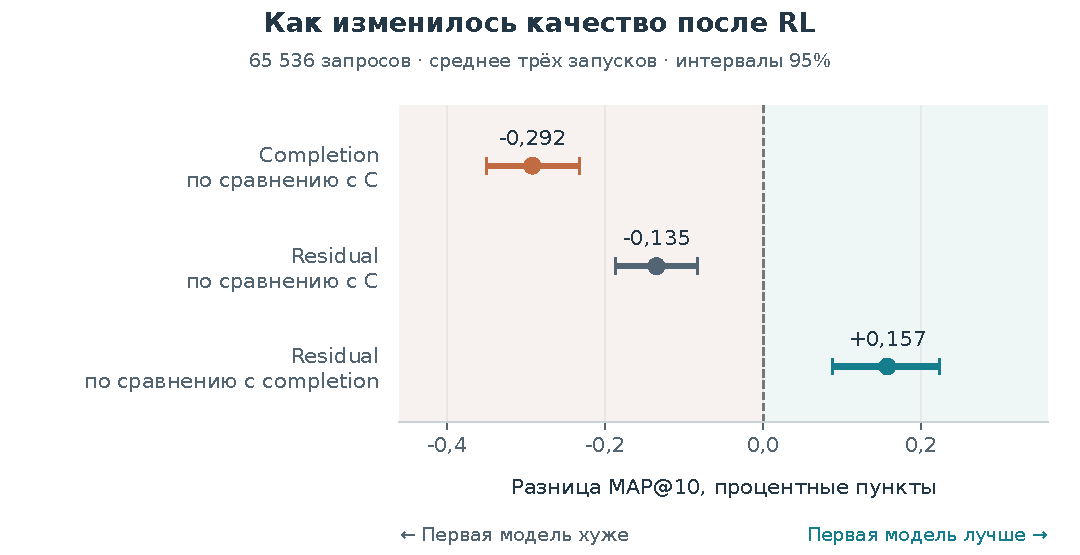
\includegraphics[width=\textwidth]{images/train-kl-and-map.pdf}
\caption{Разницы MAP@10 на 65 536 запросах, усреднённые по трём запускам с сопоставимым KL. Линии показывают 95\% доверительные интервалы по пользователям.}
\end{figure}

Интервалы учитывают различия между пользователями при фиксированных моделях, но не весь разброс повторного обучения. Выборка ранее использовалась при разработке. Сопоставимый средний KL лишь приблизительно уравнивает силу изменений.

\textbf{Прогноз досмотра вырос у обоих вариантов}

В дополнительной проверке на 1024 запросах сопоставили прогноз RM и MAP@10 на одних данных. В таблице результаты RL усреднены по трём запускам с сопоставимым KL.

\begin{center}
\begin{tabular}{lrr}
\toprule
Модель & Условный прогноз RM & MAP@10 \\
\midrule
C & 0,42065 & 0,08519 \\
Completion & 0,45058 & 0,07748 \\
Residual & 0,43063 & 0,08522 \\
\bottomrule
\end{tabular}
\end{center}

Прогноз RM взвешен вероятностью выбора и рассчитан для фильмов с наблюдениями в обучении RM. На них приходится около 97\% вероятности у всех трёх вариантов. По сравнению с C прогноз вырос примерно на 0,030 у completion и на 0,010 у residual. Это рост оценки фиксированной модели, а не измеренный рост досмотра. Точные значения и интервалы приведены в \href{https://github.com/suprend/kion-rl-recsys/blob/0154a495704c461adebc281de68d63a652946ec1/report-latex/reward1024.json}{результатах проверки RM}.

На этих 1024 запросах отличие MAP@10 residual от C не подтвердилось. Это не отменяет снижения качества, выявленного в основном сравнении на 65 536 запросах.

\textbf{Объяснение через короткие фильмы пока не подтверждено}

Проверка на 65 536 запросах для двух запусков completion не позволила установить, стала ли модель выбирать более короткие фильмы: сведения о длительности неполны.

\section{Что показали пять рекомендаций подряд}

Для 256 историй разных пользователей получили по пять рекомендаций. Сравнили исходную C и по три модели с наградами completion и residual, обученные при сопоставимом KL. На каждом шаге выбирали либо самый вероятный фильм, либо случайный фильм по вероятностям модели. Оба способа проверили с запретом повторов и без него.

Выбранный фильм добавляли в последовательность ID, после чего GPT пересчитывала её представление и оценки. Кандидаты, дополнительные признаки, время и прогнозы RM оставались такими же, как перед первым шагом. Реакцию пользователя не моделировали. Все модели были обучены выбирать один следующий фильм.

Без запрета повторов выбор самого вероятного фильма привёл к повторам во всех 256 историях у каждой модели. Из пяти рекомендаций получилось в среднем 1,6 разных фильма у C и completion и 1,8 у residual. Residual также меньше сосредотачивала выдачу на одном фильме: доля самого частого фильма среди всех рекомендаций составила около 26\% против 51\% у completion.

\begin{figure}[htbp]
\centering
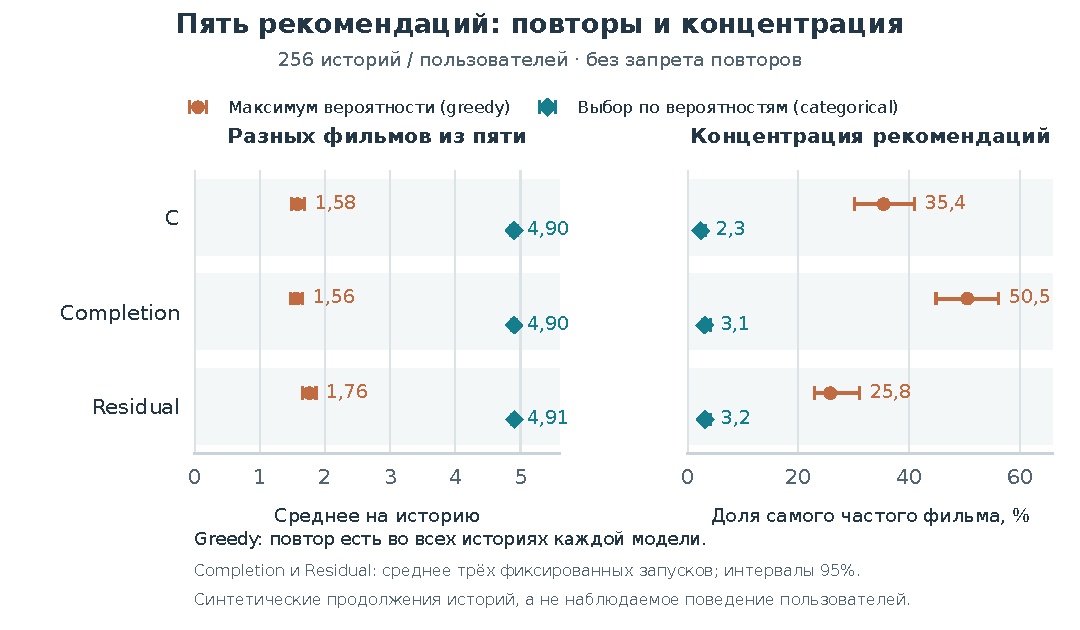
\includegraphics[width=\textwidth]{images/rollout-steps.pdf}
\caption{Пять рекомендаций без запрета повторов. Слева среднее число разных фильмов в последовательности, справа доля самого частого фильма среди всех выданных рекомендаций. Линии показывают 95\% доверительные интервалы. Результаты completion и residual усреднены по трём запускам.}
\end{figure}

При случайном выборе все три варианта дали около 4,9 разных фильма из пяти; различие residual и completion не подтвердилось. С запретом повторов каждая последовательность содержит пять разных фильмов по условию выбора.

Для последовательностей без запрета повторов также рассчитали суммарную награду. Все модели оценивали по одной шкале прогноза досмотра RM, включая residual. Из прогноза вычитали средний прогноз исходной C для начальной истории. Вес первого шага равен 1, каждого следующего в 0,9 раза меньше. Для фильмов без наблюдений в обучении RM вклад равен нулю.

\begin{center}
\begin{tabular}{lrrr}
\toprule
Способ выбора & C & Completion & Residual \\
\midrule
Самый вероятный & 0,053 & 0,419 & $-0,031$ \\
Случайный по вероятностям & 0,005 & 0,126 & 0,042 \\
\bottomrule
\end{tabular}
\end{center}

Completion получила наибольшую суммарную оценку RM, но при выборе самого вероятного фильма примерно половина всех рекомендаций приходилась на один фильм. В этом режиме residual давала несколько больше разных фильмов и меньше сосредотачивала выдачу на одном фильме, однако повторы сохранялись. При случайном выборе различие между ними по числу разных фильмов не подтвердилось. Таким образом, высокая модельная награда может сочетаться с однообразной выдачей. Повторы и концентрацию рекомендаций нужно оценивать отдельно.

Доверительные интервалы для таблицы награды не рассчитывались. Опыт проведён на историях из данных разработки.

\section{Как проверить долгосрочную пользу}

Наградой мог бы стать возврат пользователя в течение недели или число дней с просмотрами за этот период. Например, награда равна 1, если пользователь вернулся в течение семи дней после рекомендации, и 0, если не вернулся. Досмотр одного фильма можно использовать как промежуточный сигнал, но он не заменяет возвращение пользователя в сервис.

В KION есть даты взаимодействий, но повторные просмотры объединены. Поэтому по ним нельзя полностью восстановить историю посещений сервиса.

Офлайн можно оценить точность прогноза возвращения пользователя по его истории. Проверить, увеличивают ли сами рекомендации возвращаемость, можно в A/B-тесте.

\section{Приложение. Состав и расчёт признаков}

\href{https://github.com/suprend/kion-rl-recsys/blob/0154a495704c461adebc281de68d63a652946ec1/report-latex/feature-schema.json}{Реестр признаков} содержит точные названия, размеры входов и преобразования признаков каждой модели. Ниже описаны их смысл и расчёт.

\textbf{Общие правила обработки признаков}

Словари категорий и обучаемые параметры нормализации рассчитаны по обучающим данным. Остальные преобразования фиксированы. Пропуски отмечены отдельно от известных значений. Маски, вероятности и уже нормированные векторы повторно не логарифмируются.

Популярность и ItemKNN рассчитаны по прошлым взаимодействиям без текстовых и парных признаков. Даже если просмотры отобраны по дате, это не подтверждает, что сведения о фильмах были доступны в тот момент.


\newpage

\subsection{GPT: признаки фильма}

Представление фильма объединяет признаки каталога, тексты и сведения об актёрах и режиссёрах. Текстовые и обучаемые представления участников добавляются к табличным признакам.

\textbf{Каталог и серии}


\begin{longtable}{>{\raggedright\arraybackslash}p{4.1cm}>{\raggedright\arraybackslash}p{10.8cm}}
\toprule
Признак & Смысл и расчёт \\
\midrule
\endfirsthead
\toprule
Признак & Смысл и расчёт \\
\midrule
\endhead
\textbf{ID фильма} & Обучаемый вектор, соответствующий ID фильма. Общая таблица фильмов для истории и поиска кандидатов. \\[4pt]
\textbf{Жанры и страны} & Для каждого жанра и каждой страны отмечается принадлежность фильма. Одному фильму могут соответствовать несколько значений. \\[4pt]
\textbf{Тип, маркировка, студии} & Тип контента, возрастная маркировка и студии. Неизвестные значения отмечаются отдельно, в том числе для признака детского контента. \\[4pt]
\textbf{Год выпуска} & Год центрируется и масштабируется по корректным годам выпуска уникальных фильмов обучающего каталога. Пропуск отмечается отдельно. \\[4pt]
\textbf{Исходные серии} & 80 подтверждённых серий и неизвестная серия. \\[4pt]
\textbf{Ручные серии и вселенные} & Вручную размечены 81 серия и десять киновселенных. Неизвестные значения отмечаются отдельно. Эта разметка дополняет исходные 80 серий. \\[4pt]
\bottomrule
\end{longtable}

\textbf{Заполненность и доступность}


\begin{longtable}{>{\raggedright\arraybackslash}p{4.1cm}>{\raggedright\arraybackslash}p{10.8cm}}
\toprule
Признак & Смысл и расчёт \\
\midrule
\endfirsthead
\toprule
Признак & Смысл и расчёт \\
\midrule
\endhead
\textbf{Наличие текста} & Название, оригинальное название, описание, теги: индикаторы наличия. \\[4pt]
\textbf{Длина текста} & Нормализованные логарифмы числа символов и слов. \\[4pt]
\textbf{Технические метки} & 4K, сурдоперевод, тифлокомментарий, субтитры. \\[4pt]
\bottomrule
\end{longtable}

\newpage

Смысловые признаки получены из тегов и описаний по правилам и подтверждённой разметке. Упоминание в названии или теге не приравнивается к профессии героя. Если подтверждение не найдено, это ещё не означает, что признака нет. Точные состояния и метки перечислены в реестре.

\textbf{Сюжет и формат}


\begin{longtable}{>{\raggedright\arraybackslash}p{4.1cm}>{\raggedright\arraybackslash}p{10.8cm}}
\toprule
Признак & Смысл и расчёт \\
\midrule
\endfirsthead
\toprule
Признак & Смысл и расчёт \\
\midrule
\endhead
\textbf{Преодоление и выбор} & Преодоление трудностей, смена приоритетов, сильная героиня, добрые дела. \\[4pt]
\textbf{Романтические темы} & Любовный треугольник, подростковая романтика, романтические отношения, измена. \\[4pt]
\textbf{Семья и дружба} & Семейный конфликт, потеря близкого, женская и мужская дружба. \\[4pt]
\textbf{Повествовательные приёмы} & Воспоминания, закадровый рассказ, путешествие во времени, временная петля, сюрреализм, абсурдизм. \\[4pt]
\textbf{Источник сюжета} & Экранизации литературных произведений, комиксов и манги. Произведения на основе реальных событий. \\[4pt]
\textbf{Формат произведения} & Мини-сериал, самостоятельная короткая работа, антология фильма или сериала, сборник. \\[4pt]
\textbf{Запись и обучение} & Запись концерта, спектакля или стендапа. Обучающий материал. \\[4pt]
\bottomrule
\end{longtable}

\textbf{Спорт и занятия}


\begin{longtable}{>{\raggedright\arraybackslash}p{4.1cm}>{\raggedright\arraybackslash}p{10.8cm}}
\toprule
Признак & Смысл и расчёт \\
\midrule
\endfirsthead
\toprule
Признак & Смысл и расчёт \\
\midrule
\endhead
\textbf{Командный спорт} & Футбол, американский футбол, баскетбол. \\[4pt]
\textbf{Другие виды спорта} & Бокс, единоборства, бег, плавание, велоспорт, зимние виды, теннис, сёрфинг, шахматы. \\[4pt]
\textbf{Занятия} & Фитнес, йога, пилатес, растяжка, танец и балет, готовка, рыбалка, рукоделие. \\[4pt]
\textbf{Роль спорта} & Тема спорта отделена от трансляции, обучения, документального материала и игрового произведения. \\[4pt]
\bottomrule
\end{longtable}

\textbf{Профессии персонажей}


\begin{longtable}{>{\raggedright\arraybackslash}p{4.1cm}>{\raggedright\arraybackslash}p{10.8cm}}
\toprule
Признак & Смысл и расчёт \\
\midrule
\endfirsthead
\toprule
Признак & Смысл и расчёт \\
\midrule
\endhead
\textbf{Медицина и наука} & Медицинские работники, психологи, ветеринары, учителя, учёные, инженеры. \\[4pt]
\textbf{Право и служба} & Юристы, полицейские, следователи, военные, пожарные, разведчики. \\[4pt]
\textbf{Творчество} & Писатели, журналисты, музыканты, художники. \\[4pt]
\textbf{Другие профессии} & Повара, водители, пилоты, спортсмены, работники бара, бухгалтеры. \\[4pt]
\textbf{Роль профессии} & Нынешняя, прошлая, будущая и желаемая профессия, обучение, центральная роль персонажа. \\[4pt]
\bottomrule
\end{longtable}

\newpage

\textbf{Место и время действия}


\begin{longtable}{>{\raggedright\arraybackslash}p{4.1cm}>{\raggedright\arraybackslash}p{10.8cm}}
\toprule
Признак & Смысл и расчёт \\
\midrule
\endfirsthead
\toprule
Признак & Смысл и расчёт \\
\midrule
\endhead
\textbf{Места действия} & Учебные заведения, деревня, провинция, большой город, природные локации. \\[4pt]
\textbf{Учреждения} & Больница, тюрьма, гостиница, офис, военная база, лагерь. \\[4pt]
\textbf{Путь и пространство} & Судно, путешествие по дороге, космос. \\[4pt]
\textbf{Географическая роль} & Место действия и объект документального рассказа разделены. Страна производства хранится отдельно. \\[4pt]
\textbf{Календарное время} & Явные даты, интервалы, века, десятилетия, эпохи: категории, а не один угаданный год. \\[4pt]
\textbf{Временные планы} & Настоящее, будущее, воспоминания, несколько временных планов. \\[4pt]
\bottomrule
\end{longtable}

\textbf{Надёжность разметки}


\begin{longtable}{>{\raggedright\arraybackslash}p{4.1cm}>{\raggedright\arraybackslash}p{10.8cm}}
\toprule
Признак & Смысл и расчёт \\
\midrule
\endfirsthead
\toprule
Признак & Смысл и расчёт \\
\midrule
\endhead
\textbf{Состояния правил} & Найдено подтверждение признака. Данных недостаточно. Найдены противоречивые сведения. \\[4pt]
\textbf{Уточнённые состояния} & Также отрицание, случайное упоминание, отклонённый кандидат, необходимость проверки. \\[4pt]
\bottomrule
\end{longtable}

\textbf{Участники и тексты GPT}

\textbf{Актёры и режиссёры: статистика}


\begin{longtable}{>{\raggedright\arraybackslash}p{4.1cm}>{\raggedright\arraybackslash}p{10.8cm}}
\toprule
Признак & Смысл и расчёт \\
\midrule
\endfirsthead
\toprule
Признак & Смысл и расчёт \\
\midrule
\endhead
\textbf{Число участников} & Отдельно актёры и режиссёры: число, пропуски, покрытие top-100. \\[4pt]
\textbf{100 наиболее частых имён} & Отдельно для актёров и режиссёров выбираются 100 имён с наибольшим числом работ в обучающем каталоге. Имена нормализуются и объединяются внутри роли. \\[4pt]
\textbf{Другие работы} & Число других работ, отдельно фильмов и сериалов. Текущая карточка исключается. \\[4pt]
\textbf{Ранние работы} & Работы со строго более ранним годом выпуска, работы за три и пять лет. \\[4pt]
\textbf{Интервалы карьеры} & Время, прошедшее с первой и предыдущей работы, неизвестный год, другие работы того же года. \\[4pt]
\textbf{Специализация} & Жанровая и форматная специализация. Состав работ и соответствие кандидату. \\[4pt]
\textbf{Сводные показатели по участникам} & Среднее, максимум, медиана, среднее трёх наибольших значений, доступность. \\[4pt]
\textbf{Совместные работы} & Пары актёров и пары «режиссёр, актёр», повторные сотрудничества и их поддержка. \\[4pt]
\bottomrule
\end{longtable}

\textbf{Актёры и режиссёры: эмбеддинги}

Векторы актёров и режиссёров входят в представление фильма, которое используется для истории пользователя и поиска кандидатов.

\begin{longtable}{>{\raggedright\arraybackslash}p{4.1cm}>{\raggedright\arraybackslash}p{10.8cm}}
\toprule
Признак & Смысл и расчёт \\
\midrule
\endfirsthead
\toprule
Признак & Смысл и расчёт \\
\midrule
\endhead
\textbf{Эмбеддинги актёров} & Среднее обучаемых векторных представлений актёров. \\[4pt]
\textbf{Эмбеддинги режиссёров} & Среднее обучаемых векторных представлений режиссёров. \\[4pt]
\textbf{Три актёра} & Объединение в один вектор представлений трёх актёров с наибольшим числом работ в обучающем каталоге. \\[4pt]
\textbf{Редкие и отсутствующие имена} & Отдельные категории для редких и отсутствующих имён. \\[4pt]
\bottomrule
\end{longtable}

\textbf{Текстовые эмбеддинги}

Тексты преобразуются в векторы моделью \texttt{intfloat/multilingual-e5-small} (E5), которую мы использовали без дообучения. Для каждого поля рассчитывается отдельный вектор. Три обучаемых преобразования добавляют эти векторы к представлению фильма.


\begin{longtable}{>{\raggedright\arraybackslash}p{4.1cm}>{\raggedright\arraybackslash}p{10.8cm}}
\toprule
Признак & Смысл и расчёт \\
\midrule
\endfirsthead
\toprule
Признак & Смысл и расчёт \\
\midrule
\endhead
\textbf{Название} & Отдельный E5-вектор названия. \\[4pt]
\textbf{Оригинальное название} & Отдельный E5-вектор текста. \\[4pt]
\textbf{Описание} & Отдельный E5-вектор текста. \\[4pt]
\textbf{Пропуск текста} & Нулевой вектор и индикатор пропуска. Не кодируется как обычная строка. \\[4pt]
\bottomrule
\end{longtable}

\newpage

\subsection{GPT: пользователь и история}

Признаки пользователя описывают демографию, историю просмотров, активность и предпочтения. Сводные признаки входят в начальный токен BOS, а последовательность просмотренных фильмов задаётся отдельно. ID пользователя не используется как признак.

\textbf{История и демография}


\begin{longtable}{>{\raggedright\arraybackslash}p{4.1cm}>{\raggedright\arraybackslash}p{10.8cm}}
\toprule
Признак & Смысл и расчёт \\
\midrule
\endfirsthead
\toprule
Признак & Смысл и расчёт \\
\midrule
\endhead
\textbf{Просмотренные фильмы} & Идентификаторы не более 63 последних фильмов в порядке истории. Целевой фильм во вход не включается. \\[4pt]
\textbf{Возраст и доход} & Возрастные и доходные группы из исходного набора. Неизвестные значения отмечаются отдельно. \\[4pt]
\textbf{Пол и наличие детей} & Категории с неизвестным значением каждого поля. \\[4pt]
\bottomrule
\end{longtable}

\textbf{Предпочтения по каталогу}


\begin{longtable}{>{\raggedright\arraybackslash}p{4.1cm}>{\raggedright\arraybackslash}p{10.8cm}}
\toprule
Признак & Смысл и расчёт \\
\midrule
\endfirsthead
\toprule
Признак & Смысл и расчёт \\
\midrule
\endhead
\textbf{Профили атрибутов} & Доли жанров, стран, форматов, десятилетий выпуска, возрастных маркировок по последним не более чем 63 прежним взаимодействиям. \\[4pt]
\textbf{Покрытие профилей} & Число известных значений и покрытие. Для multi-hot сумма долей может превышать единицу. \\[4pt]
\bottomrule
\end{longtable}

\textbf{Активность}


\begin{longtable}{>{\raggedright\arraybackslash}p{4.1cm}>{\raggedright\arraybackslash}p{10.8cm}}
\toprule
Признак & Смысл и расчёт \\
\midrule
\endfirsthead
\toprule
Признак & Смысл и расчёт \\
\midrule
\endhead
\textbf{Давность просмотра} & Время с последнего просмотра. \\[4pt]
\textbf{Объём активности} & Число просмотренных объектов и дней с просмотрами за 1, 7 и 30 дней. \\[4pt]
\textbf{Интервалы активности} & Медиана интервалов между активными датами и их относительный разброс. \\[4pt]
\bottomrule
\end{longtable}

\textbf{Досмотр}


\begin{longtable}{>{\raggedright\arraybackslash}p{4.1cm}>{\raggedright\arraybackslash}p{10.8cm}}
\toprule
Признак & Смысл и расчёт \\
\midrule
\endfirsthead
\toprule
Признак & Смысл и расчёт \\
\midrule
\endhead
\textbf{Средний досмотр} & Среднее по корректным значениям. Пропуски и ошибочные проценты учитываются отдельно. \\[4pt]
\textbf{Пороги досмотра} & Доли значений не выше 10\% и не ниже 20, 50, 80 и 95\%. \\[4pt]
\textbf{Досмотр по группам} & Среднее, пороги 80 и 10\%, поддержка: отдельно фильмы, сериалы, последние 7 и 30 дней. \\[4pt]
\textbf{Относительный досмотр} & Вычитается сглаженный средний досмотр фильма, рассчитанный только по более ранним данным. \\[4pt]
\textbf{Остатки по атрибутам} & Отклонение среднего остатка в жанре, стране, формате и десятилетии от общего среднего пользователя. При малом числе наблюдений отклонение уменьшается. \\[4pt]
\textbf{Фоны досмотра} & Средний досмотр по типу контента и по всем объектам рассчитывается без данных текущего пользователя. \\[4pt]
\bottomrule
\end{longtable}

\newpage

\textbf{Динамика и текстовые интересы}


\begin{longtable}{>{\raggedright\arraybackslash}p{4.1cm}>{\raggedright\arraybackslash}p{10.8cm}}
\toprule
Признак & Смысл и расчёт \\
\midrule
\endfirsthead
\toprule
Признак & Смысл и расчёт \\
\midrule
\endhead
\textbf{Динамика истории} & Среднее, максимум и последнее значение показателей популярности, досмотра и интереса к связанным работам для фильмов из истории. \\[4pt]
\textbf{Профиль популярности} & Для каждого прежнего события популярность берётся до его собственного дня. \\[4pt]
\textbf{Три текстовых профиля} & Усреднение валидных E5-векторов по каждому из трёх полей и L2-нормирование. \\[4pt]
\textbf{Тексты истории} & Число доступных текстов, признаки пустого или нулевого профиля. \\[4pt]
\bottomrule
\end{longtable}

Поиск GPT сравнивает представление истории с общей таблицей фильмов скалярным произведением. Дополнительные парные признаки используются при ранжировании, а не при поиске кандидатов GPT.

\subsection{Голова A: входы поверх замороженного GPT}

Модель A использует представления истории и фильма из GPT, оценку GPT и недавнюю популярность фильма. Персонализация уже содержится в представлении истории.

\textbf{Общие входы ранкера}


\begin{longtable}{>{\raggedright\arraybackslash}p{4.1cm}>{\raggedright\arraybackslash}p{10.8cm}}
\toprule
Признак & Смысл и расчёт \\
\midrule
\endfirsthead
\toprule
Признак & Смысл и расчёт \\
\midrule
\endhead
\textbf{История GPT} & Замороженное представление истории пользователя. \\[4pt]
\textbf{Кандидат GPT} & Замороженное представление фильма. \\[4pt]
\textbf{Произведение векторов} & Покоординатное произведение представлений истории и фильма. \\[4pt]
\textbf{Оценка GPT} & Текущая оценка кандидата GPT. \\[4pt]
\textbf{Популярность за 7 дней} & Логарифм числа взаимодействий с фильмом за прежние семь дней. \\[4pt]
\bottomrule
\end{longtable}

\newpage

\subsection{Голова B: добавления к A}

Модель B использует входы A и дополнительные признаки популярности, досмотра и внешнего интереса к фильмам.

\begin{longtable}{>{\raggedright\arraybackslash}p{4.1cm}>{\raggedright\arraybackslash}p{10.8cm}}
\toprule
Признак & Смысл и расчёт \\
\midrule
\endfirsthead
\toprule
Признак & Смысл и расчёт \\
\midrule
\endhead
\textbf{Популярность} & Число пар и пользователей, доля среди просмотров. Показатели рассчитываются за всю прошлую историю и отдельно за 1, 7 и 30 дней. \\[4pt]
\textbf{Рост интереса} & Изменение популярности относительно предыдущего периода с учётом числа наблюдений. \\[4pt]
\textbf{Досмотр фильма} & Средняя доля досмотра и доли наблюдений с досмотром не выше 10\% и не ниже 20, 50, 80 и 95\%. \\[4pt]
\textbf{Доступность досмотра} & Отмечаются пропущенные и некорректные значения досмотра, а также отсутствие наблюдений. \\[4pt]
\textbf{Активность по дням недели} & Сравнение дней недели с глобальным фоном. \\[4pt]
\textbf{Интерес к участникам} & Актёры, режиссёры, студии, серии. Сама карточка исключается. Среднее, максимум, медиана, top-3. \\[4pt]
\textbf{Оценки MovieLens} & Число, среднее, сглаженное среднее оценок. Доступность сопоставления. \\[4pt]
\textbf{Wikipedia: фильм} & Просмотры статьи на русском и английском. Периоды 7 и 30 дней, рост. \\[4pt]
\textbf{Wikipedia: участники} & Статьи актёров и режиссёров на тех же языках. Периоды 7 и 30 дней, рост и агрегаты по участникам. \\[4pt]
\textbf{Внешние пропуски} & Отдельно отмечаются отсутствие статьи, неполные данные за период, отсутствие установленного соответствия и подтверждённое нулевое число просмотров. \\[4pt]
\bottomrule
\end{longtable}

Внешние данные сопоставлены с фильмами после периода наблюдения. Их доступность на момент рекомендации не проверялась.

\newpage

\subsection{Голова C: добавления к B}

Модель C использует входы B и добавляет соответствие фильма интересам пользователя, интерес к связанным работам и прогресс просмотра серии.

\begin{longtable}{>{\raggedright\arraybackslash}p{4.1cm}>{\raggedright\arraybackslash}p{10.8cm}}
\toprule
Признак & Смысл и расчёт \\
\midrule
\endfirsthead
\toprule
Признак & Смысл и расчёт \\
\midrule
\endhead
\textbf{Знакомые участники} & Актёры, режиссёры, студии и серии: доля знакомых участников, число прежних работ, покрытие истории. \\[4pt]
\textbf{Новизна режиссёра} & Сравнение режиссёра с прежней историей. \\[4pt]
\textbf{Профили интересов} & Кластеризация жанровых векторов прошлых фильмов. Соответствие одному, двум и трём профилям. \\[4pt]
\textbf{Доступность профилей} & При недостатке наблюдений или плохо разделённых группах используется меньше профилей. Отдельно отмечаются покрытие и причина уменьшения числа профилей. \\[4pt]
\textbf{Сходство текстов} & Косинусное сходство текстов кандидата с текстовыми профилями пользователя. \\[4pt]
\textbf{Работы студии и франшизы} & Объединения других карточек студии и франшизы. Просмотры и пользователи. \\[4pt]
\textbf{Динамика связанных работ} & Рост и давность связанных релизов. \\[4pt]
\textbf{Основная линия серии} & Порядок выхода подтверждённых частей основной линии серии. \\[4pt]
\textbf{Порядок релиза} & Отдельно размеченные связи между карточками по порядку выхода. Они не объединяются с порядком основной линии серии и не задают хронологию сюжета. \\[4pt]
\textbf{Известные и пропущенные части} & Известные части, недостающие предшествующие части, пропуск частей. \\[4pt]
\textbf{Продолжение и расстояние} & Ближайшее продолжение, расстояние, давность. \\[4pt]
\textbf{Полнота графа} & Полнота разметки графа. Не процент досмотра фильма. \\[4pt]
\bottomrule
\end{longtable}

A, B и C обучены независимо. Их сравнение оценивает добавленные группы признаков в совокупности, а не вклад каждого признака по отдельности.

\newpage

\subsection{Reward model: собственный набор}

CatBoost прогнозирует досмотр по демографии и истории пользователя, признакам кандидата и его ID.

\textbf{Признаки контекста}

\begin{longtable}{>{\raggedright\arraybackslash}p{4.1cm}>{\raggedright\arraybackslash}p{10.8cm}}
\toprule
Признак & Смысл и расчёт \\
\midrule
\endfirsthead
\toprule
Признак & Смысл и расчёт \\
\midrule
\endhead
\textbf{Демография} & Возрастная и доходная группы, пол, наличие детей. Неизвестные значения учитываются отдельно. \\[4pt]
\textbf{Предпочтения по каталогу} & Доли жанров, стран, типов контента, десятилетий выпуска и возрастных маркировок в истории. \\[4pt]
\textbf{Активность} & Давность просмотра, число просмотренных объектов и дней с просмотрами за 1, 7 и 30 дней. Медиана и относительный разброс интервалов между активными датами. \\[4pt]
\textbf{Досмотр в истории} & Среднее и доли досмотров не выше 10\% и не ниже 20, 50, 80 и 95\%. Для фильмов, сериалов, последних 7 и 30 дней отдельно рассчитаны среднее и доли по порогам 10 и 80\%. \\[4pt]
\textbf{Относительный досмотр} & Досмотр относительно фона фильма. Отклонения по жанрам, странам, типам контента и десятилетиям, с учётом числа наблюдений. \\[4pt]
\textbf{Динамика истории} & Среднее, максимум и последнее значение локальной динамики фильмов из истории. Число и доля фильмов с доступными данными. \\[4pt]
\bottomrule
\end{longtable}

\textbf{Признаки кандидата}

\begin{longtable}{>{\raggedright\arraybackslash}p{4.1cm}>{\raggedright\arraybackslash}p{10.8cm}}
\toprule
Признак & Смысл и расчёт \\
\midrule
\endfirsthead
\toprule
Признак & Смысл и расчёт \\
\midrule
\endhead
\textbf{Базовый каталог} & Жанры, страны, тип контента, год выпуска и возрастная маркировка. \\[4pt]
\textbf{Статические признаки} & Студии, подтверждённые серии, признак детского контента. Наличие и длина текстов, 4K, сурдоперевод, тифлокомментарий и субтитры. \\[4pt]
\textbf{Статистика участников} & Число актёров и режиссёров, наиболее частые имена, другие и более ранние работы, интервалы карьеры, специализация и совместные работы. Также рассчитываются сводные показатели по всему составу участников. \\[4pt]
\textbf{Смысловые признаки} & Сюжетные темы, повествовательные приёмы, источник сюжета, формат, спорт и занятия, профессии, место и время действия. Отдельно учитывается надёжность разметки. \\[4pt]
\textbf{Динамика кандидата} & Популярность, рост интереса, досмотр, активность по дням недели и интерес к участникам, студиям и сериям. Отдельно учитываются доступность данных и число наблюдений. \\[4pt]
\textbf{ID фильма} & Отдельный категориальный признак. \\[4pt]
\bottomrule
\end{longtable}

\newpage

\section{Приложение. Условия эксперимента}

\textbf{Периоды обучения и оценки}

Все даты в таблице относятся к 2021 году. «До» означает строго раньше указанного дня; диапазоны включают обе границы.

\begin{longtable}{>{\raggedright\arraybackslash}p{3.6cm}>{\raggedright\arraybackslash}p{2.8cm}>{\raggedright\arraybackslash}p{8.1cm}}
\toprule
Этап & Период & История и статистика \\
\midrule
\endfirsthead
\toprule
Этап & Период & История и статистика \\
\midrule
\endhead
Обучение GPT & До 9 августа & История до дня целевого просмотра. \\[4pt]
Обучение A/B/C & До 9 августа & История и динамика до дня запроса. GPT обучен на всей обучающей части. \\[4pt]
Обучение RM & До 2 августа & История до дня цели; статистики и преобразования по данным до 2 августа. \\[4pt]
Выбор версии RM & 2–8 августа & История и статистика по данным до 2 августа. \\[4pt]
Калибровка RM & 2–8 августа & История и статистика по данным до 2 августа. Пользователи не пересекаются с группой выбора версии. \\[4pt]
Оценка RM & 9–15 августа & История до 9 августа; динамические признаки кандидата и обученные статистики до 2 августа. \\[4pt]
Обучение RL & 2–8 августа & История до даты состояния. Готовые GPT, C и калиброванная RM фиксированы. \\[4pt]
Общее сравнение моделей & 9–15 августа & История, динамика и кандидаты до 9 августа; недельная популярность за 2–8 августа. \\[4pt]
Тестовая часть & 16–22 августа & В приведённое сравнение не входит. \\
\bottomrule
\end{longtable}

Для некоторых обучающих состояний RL веса GPT и ранкера, а также калибровка RM используют сведения из более поздних дней. Поэтому опыт сравнивает заранее подготовленные модели, а не воспроизводит работу сервиса на каждую историческую дату.


\textbf{Обучение и сопоставление моделей}

Каждый запуск RL включал 1000 обновлений на 512 историях. Между тремя парами запусков менялась последовательность выбора обучающих примеров; данные, начальные веса и остальные настройки сохранялись. Для completion коэффициент KL-штрафа равен \(\beta=0{,}5\), для residual \(\beta\approx0{,}1627\). Во всех парах отношение среднего KL residual к среднему KL completion на обучающих историях находилось в заданном диапазоне от 0,8 до 1,2. Результаты трёх моделей усредняются с равными весами; это не ансамбль.

Калибровка RM подбирает линейную поправку к прогнозу, ограниченному диапазоном [0; 1]. Она практически не изменила RMSE: 0,35204 после поправки против 0,35201 до неё. Контрольный прогноз из раздела 4 усредняет исторические средние досмотров фильма и пользователя, сглаженные к общему среднему. Подробности сохранены в \href{https://github.com/suprend/kion-rl-recsys/blob/0154a495704c461adebc281de68d63a652946ec1/evidence/fullstudy/rm-evaluation-metrics.json}{оценке RM}.

\textbf{Формула награды}

Вероятности выбора получены softmax от оценок ранкера с температурой 1:
\[
\pi_\theta(i\mid s)=\operatorname{softmax}_i z_\theta(s,i).
\]
Веса обновляются методом Adam по градиенту следующей цели, рассчитанной по всем 1024 кандидатам:
\[
\max_\theta\;\mathrm{E}_s\!\left[\sum_i\pi_\theta(i\mid s)a(s,i)
-\beta D_{\mathrm{KL}}(\pi_\theta(\cdot\mid s)\Vert\pi_C(\cdot\mid s))\right].
\]
Здесь \(a(s,i)\) есть награда за вычетом её среднего под исходной C. Это среднее рассчитывается только среди фильмов с наблюдениями в обучении RM: взвешенная сумма наград делится на суммарную вероятность этих фильмов. Центрирование выполняется отдельно для completion и residual. Для остальных кандидатов \(a=0\), но они остаются в softmax и KL. Награда рассчитывается из прогноза RM; сам прогноз не добавляется ко входам ранкера.

\textbf{Расчёт оценок}

Парные 95\% доверительные интервалы получены по 2000 общим bootstrap-выборкам пользователей: каждый выбранный пользователь включается со всеми его запросами. Метрики пересчитываются для каждой выборки. Для каждого варианта RL результаты усредняются по трём фиксированным запускам. Запуски обучения не перевыбираются; поправка на множественные сравнения не применяется. Сопоставимый средний KL не гарантирует одинаковых изменений для каждой истории и сам по себе не устанавливает причинный эффект выбора награды.

На 1024 запросах условный прогноз RM равен взвешенной сумме прогнозов для фильмов с наблюдениями в обучении RM, делённой на суммарную вероятность их выбора. При bootstrap числитель и знаменатель пересчитываются вместе. Это отдельная проверка награды, а не оценка на всех 65 536 запросах.

В пятишаговой проверке доля самого частого фильма сначала рассчитывается для каждой модели, затем усредняется по трём запускам. При случайном выборе использована одна общая фиксированная последовательность случайных чисел для каждой истории; интервалы не учитывают разброс при повторном случайном выборе. Запрет повторов исключает только фильмы, уже выданные в текущей последовательности.

Суммарная награда за пять шагов использует одну шкалу прогноза досмотра для всех моделей, включая residual. Прогноз центрирован относительно C на начальной истории; вес каждого следующего шага уменьшается в 0,9 раза. Для фильмов без наблюдений в обучении RM вклад равен нулю, такие последовательности не исключаются. Это оценка выбранных фильмов, а не ожидание по всем кандидатам. Формула и значения сохранены в \href{https://github.com/suprend/kion-rl-recsys/blob/0154a495704c461adebc281de68d63a652946ec1/report-latex/rollout-reward256.json}{расчёте награды}, метрики выдачи в \href{https://github.com/suprend/kion-rl-recsys/blob/0154a495704c461adebc281de68d63a652946ec1/report-latex/rollout256.json}{результатах генерации}.

\textbf{Проверка длительности}

На 65 536 запросах сравнили два запуска completion с C, каждый отдельно. Для каждого запроса вероятности нормировали по всем фильмам в пуле, включая фильмы с неизвестной длительностью. По этим весам сравнивали геометрические средние длительности, а не среднее время реального просмотра.

Для известных фильмов использовали интервалы длительности из источников, для неизвестных проверили два диапазона возможных значений. Если неизвестные длительности лежат от 1 до 1440 минут, сокращение геометрического среднего на 5\% и более исключается. При диапазоне от 0,1 до 10 080 минут оно уже не исключается. Сокращение на 1\% и более не исключается в обоих случаях. Эти границы отражают неопределённость метаданных, а не статистический доверительный интервал. Метаданные произведения также не удостоверяют длительность его версии в KION в 2021 году. Точные расчёты сохранены в \href{https://github.com/suprend/kion-rl-recsys/blob/0154a495704c461adebc281de68d63a652946ec1/report-latex/duration-summary.json}{проверке длительности}.

\section{Материалы и воспроизведение}

\href{https://github.com/suprend/kion-rl-recsys/blob/0154a495704c461adebc281de68d63a652946ec1/reproduction/saved_metrics64k.py}{Программа пересчёта} воспроизводит метрики на 65 536 запросах и парные доверительные интервалы по сохранённым рангам и группам пользователей, без запуска моделей: результаты совпали с точностью до численной погрешности. \href{https://github.com/suprend/kion-rl-recsys/blob/0154a495704c461adebc281de68d63a652946ec1/REPRODUCING.md}{Инструкция}, \href{https://github.com/suprend/kion-rl-recsys/blob/0154a495704c461adebc281de68d63a652946ec1/source/README.md}{код}, \href{https://github.com/suprend/kion-rl-recsys/blob/0154a495704c461adebc281de68d63a652946ec1/reports/REPORT.md}{дополнительные результаты}, \href{https://github.com/suprend/kion-rl-recsys/blob/0154a495704c461adebc281de68d63a652946ec1/reports/LIMITATIONS.md}{ограничения} и \href{https://github.com/suprend/kion-rl-recsys/blob/0154a495704c461adebc281de68d63a652946ec1/evidence/INDEX.json}{индекс данных} доступны по ссылкам на закреплённую версию репозитория GitHub. Веса и входные данные предоставляются отдельно. Пересчёт не воспроизводит подготовку данных и обучение; полный запуск на новой машине не проверялся.

% REPORT_BODY_END

\end{document}
